%\documentclass[onecolumn,draftcls]{IEEEtran}
%\documentclass[journal,twocolumn,10pt,letter]{IEEEtran}
\documentclass[conference,10pt,twocolumn,letter]{IEEEtran}
%\documentclass[journal,onecolumn,12pt,doublespace]{IEEEtran}
%\documentclass[journal,onecolumn,11pt,draftcls,doublespace]{IEEEtran}
%\documentclass[journal,onecolumn]{IEEEtran}
\IEEEoverridecommandlockouts
\ifCLASSINFOpdf
\else
\fi
\usepackage{algorithm}
\usepackage[noend]{algpseudocode}
\usepackage[cmex10]{amsmath}
\usepackage{amsthm}
\usepackage{amssymb}
\usepackage{mathrsfs}
\usepackage{amsbsy}
\usepackage{mathrsfs}
\usepackage{setspace}
\usepackage{graphicx}
\usepackage{caption}
\usepackage{subcaption}
\usepackage{psfrag}
\usepackage{newclude}
\usepackage[normalem]{ulem}
\usepackage{latexsym}
%\usepackage{tikz}
\usepackage[table]{xcolor}
\usepackage{multirow}
\usepackage{rotating}
\usepackage{booktabs}
\usepackage{amsmath}
\usepackage{mathrsfs}
\usepackage{bbm} % indicator function
\usepackage{filecontents}
\usepackage{amsmath,epsfig,cite,amsfonts,amssymb,psfrag,subfig}
\def\CE{\mathcal{E}}
\def\A{{A^n_\epsilon}}
\def\bS{{\boldsymbol{S}}}
\def\bs{{\boldsymbol{s}}}
\def\bz{{\boldsymbol{z}}}
\def\bu{{\boldsymbol{u}}}
\def\bv{{\boldsymbol{v}}}
\def\bU{{\boldsymbol{U}}}
\def\bx{{\boldsymbol{x}}}
\def\bX{{\boldsymbol{X}}}
\def\by{{\boldsymbol{y}}}
\def\bY{{\boldsymbol{Y}}}
\def\pr{{\text{P}}}
\def\c{{\mathcal{C}}}
%%%%%%%%%%%%%%%%% Define \doublehat
\usepackage{accents}
\newlength{\dhatheight}
\newcommand{\doublehat}[1]{%
    \settoheight{\dhatheight}{\ensuremath{\hat{#1}}}%
    \addtolength{\dhatheight}{-0.35ex}%
    \hat{\vphantom{\rule{1pt}{\dhatheight}}%
    \smash{\hat{#1}}}}
%%%%%%%%%%%%%%%%%%% Define Independent Symbol
\newcommand\independent{\protect\mathpalette{\protect\independenT}{\perp}}
\def\independenT#1#2{\mathrel{\rlap{$#1#2$}\mkern2mu{#1#2}}}
%%%%%%%%%%%%%%%%%%%%%%%%%%%
\allowdisplaybreaks
\newtheorem{remark}{Remark}
\newtheorem{theorem}{Theorem}
\newtheorem{lemma}{Lemma}
\newtheorem{proposition}{Proposition}
\newtheorem{corollary}{Corollary}
\graphicspath{{figures/}}
\allowdisplaybreaks
\newcommand{\eqdef}{\overset{\mathrm{def}}{=\joinrel=}}
\hyphenation{op-tical net-works semi-conduc-tor}
%%%%%%%%%%%%%%%%%%%%%%%%%%%%%%%%%%%%%%%%%%%%%%%%%%%%%%%%%%%%%%%%%%%%%%%%%%%%%%%%%%%%%%%%%%%%%%%%%%%%%%%%%%%%%%%%%%%%%%%%%%%%%%%%%%%%
\begin{document}
\title{Optimal Power Allocation for Distributed MIMO C-RAN System with Limited Fronthaul Capacity} \author{\IEEEauthorblockN{\normalsize
     Mojdeh Karbalaee Motalleb, Amirreza Kabiri, Mohammad Javad Emadi}
  \IEEEauthorblockA{\small Electrical Engineering Department, Amirkabir University of Technology, Tehran, Iran\\
    E-mails: \{mkm1992, a.r.kabiri, mj.emadi\}@aut.ac.ir}
    \vspace{-.75cm}
    }
\maketitle
%%%%%%%%%%%%%%%%%%%%%%%%%%%%%%%%%%%%%%%%%%%%%%%%%%%%%%%%%%%%%%%%%%%%%%%%%%%%%%%%%%%%%%%%%%%%%%%%%%%%%%%%%%%%%%%%%%%%%%%%%%%%%%%%%%%%
\begin{abstract}
This paper investigates the optimal power allocation for the downlink of multiple-input multiple output (MIMO) cloud radio access network (C-RAN) with limited fronthaul capacity in terms of maximizing energy efficiency (EE). 
In the considered system, the compressed and precoded message generated by Central Unit (CU) is transmitted to Remote Radio Heads (RRHs) via a fronthaul link with limited capacity, and the RRHs and users equipments (UEs) are assumed to be clustered into $S$ cluster set.
Here, we used an iterative algorithm with Lagrangian function to optimize the EE.
%Karush-Kuhn-Tucker (KKT) conditions
 \emph{index Terms}- Coud Radio Access Network, Multiple-Input Multiple Output, Energy efficincy, Clusterization, Power allocation, Karush-Kuhn-Tucker (KKT) conditions.
\end{abstract}
\IEEEpeerreviewmaketitle
%%%%%%%%%%%%%%%%%%%%%%%%%%%%%%%%%%%%%%%%%%%%%%%%%%%%%%%%%%%%%%%%%%%%%%%%%%%%%%%%%%%%%%%%%%%%%%%%%%%%%%%%%%%%%%%%%%%%%%%%%%%%%%%%%%%%
\section{Introduction}
The growing demand of higher data rates led vendors to think of the next generation of wireless networks which will essentially provide higher throughputs and more coverage than the state-of-art technologies. There are some new concepts introduced to enhance 5G networks such as; Het-Net systems, mmWave communications, Large-scale MIMO systems, and Cloud-Radio Access Networks. Each of the above mentioned concepts fulfills different requirements of 5G networks. As the main focus of this paper is on the C-RAN technology, it is briefly introduced next. In C-RAN systems, in order to have a more efficient system in terms of computational resources, baseband processings, which may have high computational complexities, are transfered from base stations to control centers located in a cloud. In addition to managing computational resources, C-RAN technology can provide new concepts such as co-operation among RRHs, RRH clustering \cite{33,55}. To obtain both advantages of C-RAN and MIMO system, using MIMO C-RAN system simultaneously can enhance achievable rate and also EE \cite{33}. By using MIMO system, we can achieve higher data rates and even better EE compared to conventional systems by exploiting multiple number of antennas to transmit or receive data streams.


In order to consider feasible links between CU and RRHs, named as fronthaul, the capacities of these inks are assumed to be limited \cite{22,44,1111,66}. As a result of limited fronthaul the messages passed through these links need to be compressed \cite{22,44,1111,66} . One of the main problems that now has attracted the attention of researches in MIMO C-RAN systems is how to efficiently perform detections or precodings and compressions of messages before transmitting them to CU or RRHs. Deploying efficient resource allocations causes prevention of wasting energy and as a result leads to higher EE \cite{33,55,77}. In\cite{22,44,1111,66}, the authors investigated optimizing achievable rate according to the precoding and power matrix and quantization noise with fronthaul capacity constraint. In \cite{66}, the approach of CFE (Compress-Forward Estimate) in uplink (UL) and improving data rates is investigated by using ECF (Estimate-Compress-Forward) instead can reach better performance in system, where RRH, estimate CSIT in UL, compress message and forward it to CUs studied.


In this paper, the downlink of a MIMO C-RAN system is considered where CU precodes the message, compresses the resulting signals. The compressed version of signal is forwarded via the limited capacity fronthaul links to the RRHs. it is assumed that RRHs and UEs are clustered in a way that certain clusters RRHs serve certain groups of UEs. In such system the knowledge of Channel State Information at Transmitter side (CSIT) is needed to compute precoding matrices. Since CSIT is imperfectly obtained from uplink pilot transmissions we assume that the CSIT is obtained with a certain error. MMSE precoding is applied to reduce interference and enhance the performance of the system.

\begin{figure}
  \centering
    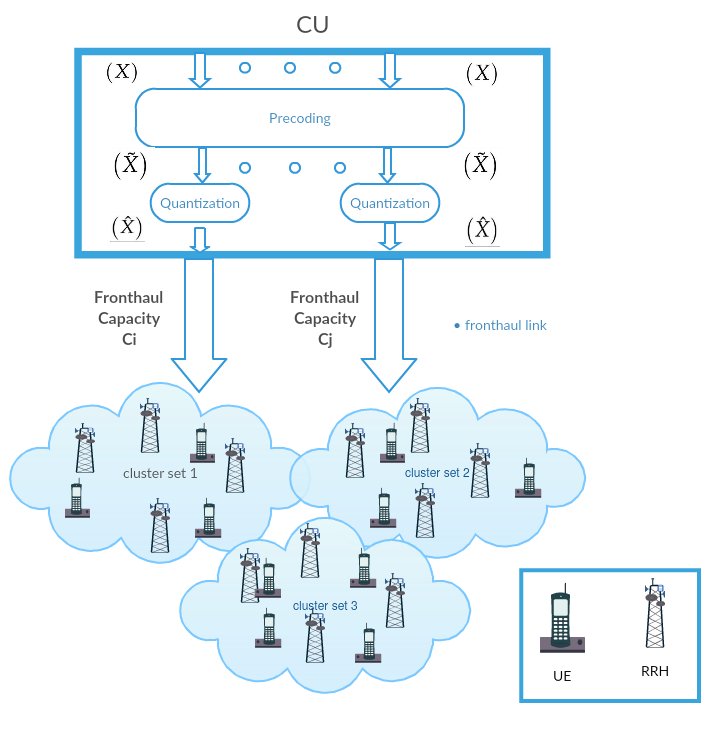
\includegraphics[width=8cm, height=8cm]{c1}
  \caption{Cooperative MIMO downlink C-RAN system.}
  \label{fig:c11}
\end{figure}

\section{System Model and Problem Formulation}

In this section, the system model, achievable rate and the main problem which is optimizing power allocation is expressed.

\subsection{System Model}

Downlink of a MIMO C-RAN system consists of $R$ RRHs serving $D$ single antenna user equipments (UE) is considered. It is assumed that RRHs and UEs are clustered in to $S$ cluster set in a way that the $v$-th cluster set, has $R_v$ RRHs serving ${D}_v$ UEs. Furhtermore, it is assumed that the $j$-th RRH in the $v$-th cluster is connected to CU via a optical fibers with limited capacity of $c_{r_{(v,j)}}$. Each user receives both intra-cluster and inter-cluster interferences. So we have
\begin{equation}
\begin{split}
\mathcal{R}_v= \{  r_{(v,i)} | 1 \leq i \leq {R}_v , i\in Z^+\}, \\
\mathcal{C}_{\mathcal{R}_v}= \{c_{r_{(v,j)}}| 1 \leq j \leq {R}_v , j\in Z^+\}, \\
\mathcal{D}_v= \{  d_{(v,k)} | 1 \leq k \leq {D}_v , k\in Z^+\},  \\
\end{split}
\end{equation}
where $\mathcal{R}_v$, $\mathcal{C}_{\mathcal{R}_v}$, and $\mathcal{D}_v$ respectively represent the RRH set, the capacity set and the UE set  for the $v$-th cluster set.
In CU we apply the approach of compressing after precoding and then forwarding.
\subsection{Achievable Rate Analysis}
In this subsection, the achievable data rate of the considered system is investigated. 
\begin{theorem}\label{t1}
The achievable data rate for UE $d_{(s,k)}$ is
\begin{equation}\label{e1}
\mathfrak{R}_{d_{(s,k)}} = B \log_2(1+\gamma_{d_{(s,k)}}),
\end{equation}
where, $B$ is the channel bandwidth and $\gamma_{d_{(s,k)}}$ is the received SINR for the $k$-th UE in the $s$-th cluster set formulated as follows
\begin{equation}\label{5}
\gamma_{d_{(s,k)}}= \frac{p_{d_{(s,k)}}|\boldsymbol{h}_{\mathcal{R}_s, d_{(s,k)}}^H \boldsymbol{w}_{\mathcal{R}_{s},d_{(s,k)}}|^2}{I_{d_{(s,k)}}+BN_0}.
\end{equation}
In \eqref{5}, $I_{d_{(s,k)}}$, denotes the power od interfering signals, $N_0$ represents the noise power, $\boldsymbol{h}_{\mathcal{R}_s, d_{(s,k)}}$ shows the channel gain vector between the $k$-th UE in the $s$-th cluster set and $\boldsymbol{w}_{\mathcal{R}_{s},d_{(s,k)}}$ indicates the precoding vector used in $s$-th cluster set for the $k$-th UE.
$p_{d_{(s,k)}}$ is the power RRHs that transmit to the $k$-th UE in the $s$-th cluster set.
\end{theorem}

\begin{proof}
%%%%%%%%%%%%%
Let $\boldsymbol{y}_{\mathcal{D}_s}$ be a $D_s \times 1$ vector denoting the received signals by the set of UEs in the $s$-th cluster which is demonstrated as 
\begin{equation} \label{1}
\boldsymbol{y}_{\mathcal{D}_s} = \sum_{v=1}^S \boldsymbol{H}^H_{\mathcal{R}_v,\mathcal{D}_s}\hat{\boldsymbol{x}}_{\mathcal{R}_v}+ \boldsymbol{z}_{\mathcal{D}_s},
\end{equation}
where $\hat{\boldsymbol{x}}_{ \mathcal{R}_v} = [\hat{x}_{ r_{(v,1)}},...,\hat{ x}_{ r_{(v,\mathcal{R}_v)}}]^T \in \mathbb{C}^{{R}_v } $ is the transmitted message vector for the $v$-th cluster set, $\boldsymbol{z_{\mathcal{D}_s}} \backsim \mathcal{N}(0,N_0\boldsymbol{I}_{{D}_s})$ shows the additive white Guassian noise with the power of $N_0$, and $\boldsymbol{H}_{\mathcal{R}_v,\mathcal{D}_s}=\left[\boldsymbol{h}_{\mathcal{R}_v,d_{(s,1)}},\ldots,\boldsymbol{h}_{\mathcal{R}_v,d_{(s,\mathcal{D}_s)}}\right]^T  \in \mathbb{C}^{{R}_v\times {D}_s}$ 
represents the channel matrix between RRH set $\mathcal{R}_v$ to UE set
$\mathcal{D}_s$. The channel vector from the RRH cluster $v$ to the $k$-th UE in the $s$-th cluster set $\boldsymbol{h}_{\mathcal{R}_v,d_{(s,k)}}\in \mathbb{C}^{{R}_v}$ is modeled as follows
\begin{equation}
\boldsymbol{h}_{\mathcal{R}_v,d_{(s,k)}} = \boldsymbol{\beta}^\frac{1}{2}_{\mathcal{R}_v,d_{(s,k)}} \boldsymbol{g}_{\mathcal{R}_v,d_{(s,k)}},
\end{equation}
% resizebox{0.3\hsize}{!}{$
where \resizebox{0.35\hsize}{!}{$\boldsymbol{g}_{\mathcal{R}_v,d_{(s,k)}} \backsim \mathcal{N}(0,N_0\boldsymbol{I}_{\mathcal{D}_s})$} represents the fast fading channel vector and \resizebox{0.75\hsize}{!}{$\boldsymbol{\beta}_{\mathcal{R}_v,d_{(s,k)}}=\text{diag}(a_{r_{(v,1),d_{(s,k)}}},\ldots,a_{r_{(v,\mathcal{R}_v),d_{(s,k)}}})$}
indicates the large scale fading matrix \cite{88}. In addition, the transmitted signal has the following form
\begin{equation}
\label{eq_pow1}
 \hat{\boldsymbol{x}}_{\mathcal{R}_v} = \tilde{\boldsymbol{x}}_{\mathcal{R}_v} + \boldsymbol{Q}_{\mathcal{R}_v},
\end{equation}
where, $\boldsymbol{Q}_{\mathcal{R}_v} = \left[ q_{r_{(v,1)}},\ldots,q_{r_{(v,R_v)}}\right]^T$,  is the quantization noise vector originating from compression made after precoding in the CU with element distribution of
$q_{M_{(t,i)}}\backsim \mathcal{N}(0,\sigma_{q_{(t,i)}}^2) $. Moreover,
$$\tilde{\boldsymbol{x}}_{\mathcal{R}_v} = \textbf{W}_{\mathcal{R}_v,\mathcal{D}_v} \textbf{P}_{\mathcal{D}_v}^{\frac{1}{2}} \boldsymbol{x}_{ \mathcal{D}_v},$$
denotes the precoded message before compression.


As mentioned before, channel vector is assumed to be known with errors, the imperfection of channel estimation is modeled as follows
\begin{equation*}
\hat{\boldsymbol{h}}_{\mathcal{R}_v,d_{(s,k)}} = \boldsymbol{h}_{\mathcal{R}_v,d_{(s,k)}} + \Delta \boldsymbol{h}_{\mathcal{R}_v,d_{(s,k)}},
\end{equation*}
$\Delta \boldsymbol{h}_{\mathcal{R}_v,d_{(s,k)}}$ denotes the estimation error vector with a Guassian distribution of
$$\Delta \boldsymbol{h}_{\mathcal{R}_v,d_{(s,k)}}\backsim \mathcal{N}(0,\boldsymbol{\phi}_{\mathcal{R}_v,d_{(s,k)}}^2),$$
where 
$$\boldsymbol{\phi}_{\mathcal{R}_v,d_{(s,k)}} = \text{diag}(\phi_{r_{(v,1)},d_{(s,k)}},\ldots,\phi_{r_{(v,\mathcal{R}_v)},d_{(s,k)}}).$$


By using MMSE precoding, the precoding matrix is expressed as follows
\begin{equation}
\boldsymbol{W}_{\mathcal{R}_s,\mathcal{D}_s} = \hat{\boldsymbol{H}}_{\mathcal{R}_s,\mathcal{D}_s}(\hat{\boldsymbol{H}}_{\mathcal{R}_s,\mathcal{D}_s}^H \hat{\boldsymbol{H}}_{\mathcal{R}_s,\mathcal{D}_s}+ \alpha \boldsymbol{I}_{{D}_s})^{-1},
\end{equation} 
where, $\alpha$ is the regularization factor.


Then the before mentioned $I_{d_{(s,k)}}$, denoting the interference power, can be written as follows
\begin{equation}\label{6}
\begin{split}
I_{d_{(s,k)}} &=  \underbrace{\sum_{\substack{l=1 \\ l\neq k}}^{{D}_s} |\boldsymbol{h}_{\mathcal{R}_s, d_{(s,k)}}^H \boldsymbol{w}_{\mathcal{R}_{s},d_{(s,l)}}|^2  p_{d_{(s,l)}}}_{\text{(intra-cluster interference)}}\\
&+\underbrace{\sum_{\substack{v=1 \\ v\neq s}}^{S} \sum_{l=1}^{{D}_s} |\boldsymbol{h}_{\mathcal{R}_v, d_{(s,k)}}^H \boldsymbol{w}_{\mathcal{R}_{v},d_{(v,l)}}|^2 p_{d_{(v,l)}}}_{\text{(inter-cluster interference)}}\\
& +\underbrace{ \sum_{v=1}^{S} \sum_{i=1}^{{R}_v} {\sigma_q}_{r_{(v,i)}}^2 \sum_{l=1}^{{D}_s} |\boldsymbol{h}_{r_{(v,i)}, d_{(v,l)}}^H|^2 }_{\text{(quantization noise interference)}}.
\end{split}
\end{equation}

 \end{proof}
\section{Optimizing Power Allocation}
Let the power of transmitted signal by the $i$-th RRH in the $s$-th cluster set indicated by
\begin{equation} \label{eq_pow2}
\bar{p}_{r_{(s,i)}} = \frac{1}{T} \mathit{E}[|| \hat{x}_{\mathcal{D}_v} ||^2] ,
\end{equation}
where $T$ is the symbol duration assumed to be 1 throughout the paper. By plugging eq (\ref{eq_pow1}) into eq (\ref{eq_pow2}), the power of transmitted signal has the following form
\begin{equation}
\bar{p}_{r_{(s,i)}} = \boldsymbol{w}_{r_{(s,i)},\mathcal{D}_{s}} \boldsymbol{P}_{\mathcal{D}_v}^{\frac{1}{2}} \boldsymbol{P}_{\mathcal{D}_v}^{H \frac{1}{2}}   \boldsymbol{w}_{r_{(s,i)},\mathcal{D}_{s}}^H + \sigma_{q_{(s,i)}}^2.
\end{equation}
As a result the achievable rate on the fronthual link between the CU and the $i$-th RRH in $t$-th cluster should be higher than
\begin{equation}
C_{R_{(t,i)}} = \log{(1+\frac{w_{r_{(s,i)},\mathcal{D}_{s}} \boldsymbol{P}_{\mathcal{D}_v}^{\frac{1}{2}} \boldsymbol{P}_{\mathcal{D}_v}^{H \frac{1}{2}}   w_{r_{(s,i)},\mathcal{D}_{s}}^H }{ \sigma_{q_{(s,i)}}^2})},
\end{equation}
in order to be able to transmit the aforementioned signals via fronthual links.
\subsection{Problem Statement}
The ratio of the sum-rate of system to the total power transmitted by RRHs indicates one of the most pormising indicators for selecting new technologies, named as the energy efficiency of system and denoted by $\eta$, which can be formulated as
\begin{equation}\label{eta}
\eta(\boldsymbol{P}) := \frac{\sum\limits_{s=1}^{S} \sum\limits_{k=1}^{{D}_s}\mathfrak{R}_{d_{(s,k)}} }{\sum\limits_{s=1}^{S} \sum\limits_{i=1}^{{R}_s}\bar{p}_{r_{(s,i)}}} = \frac{R_{total}(\boldsymbol{P})}{P_{RRH}(\boldsymbol{P})},
\end{equation}
in which $ \boldsymbol{P} = \{ \boldsymbol{P}_{\mathcal{D}_s}|  1 \leq s \leq S, s \in \mathbb{Z}^{+} \}$ is a power allocation matrix.
In this paper, maximization of energy efficiency is investigated with the presence of following constraints, 
\begin{equation}\label{p1}
\begin{aligned}
\max\limits_{\boldsymbol{P}}   \quad &   \eta(\boldsymbol{P})\\
\text{subject to} \quad  & \bar{p}_{r_{(s,i)}} \leq P_{max} && \qquad \forall s, \forall i,   \\
&\mathfrak{R}_{d_{(s,k)}} \geq  \mathfrak{R}_{d_{(s,k)}}^{th} && \qquad \forall s, \forall k, \\
&C_{r_{(s,i)}} \leq C_{r_{(s,i)}}^{th}  &&\qquad \forall s, \forall i, \\
&p_{d_{(s,k)}}  \geq 0                                  &&\qquad \forall s, \forall k, \\
\end{aligned}			
\end{equation}
Since the problem is not a convex problem, an iterative algorithm is used to derive the optimal values for the maximization problem. 
\subsection{Proposed Method}
In this subsection, instead of maximizing eq \eqref{eta}, we solve an equivalent problem by using an iterative algorithm. 
\begin{theorem}\label{t2}
 $\eta^*$ can be obtained if and only if 
\begin{equation}\label{q2}
\begin{split}
&\max \limits_{\boldsymbol{P}} (R_{total}(\boldsymbol{P}) - \eta^* P_{RRH}(\boldsymbol{P}))=\\
& R_{total}(\boldsymbol{P}^*) - \eta^* P_{RRH}(\boldsymbol{P}^*) =0,
\end{split}
\end{equation}
where $\{\boldsymbol{P}\}$ would be a feasible solution of problem \eqref{p1}.
\end{theorem}
\begin{proof}
See Theorem (1) in \cite{11}.
\end{proof}

To solve this problem, we use Lagrangian function  by an iterative algorithm proposed in \cite{11}.
For simplicity, the upper bound for the interference is considered as follows
\begin{equation}
\begin{split}
\tilde{I}_{d_{(s,k)}} &= \sum_{v=1}^{S} P_{max}|| \boldsymbol{h}_{\mathcal{R}_v,d_{(s,k)}} \boldsymbol{w}_{\mathcal{R}_v,d_{(s,k)}}||^2 ,\\
& +  \sum_{v=1}^{S} \sum_{i=1}^{{R}_v} {\sigma_q}_{r_{(v,i)}}^2 \sum_{l=1}^{{D}_s} |\boldsymbol{h}_{r_{(v,i)}, d_{(v,l)}}^H|^2.
\end{split}
\end{equation}
So the following lower band for eq \eqref{e1} is used for finding optimal values
\begin{equation}\label{e11}
\mathfrak{\tilde{R}}_{d_{(s,k)}} = B \log_2(1+\tilde{\gamma}_{d_{(s,k)}}),
\end{equation}
where $\tilde{\gamma}_{d_{(s,k)}}$ is
\begin{equation}\label{15}
\tilde{\gamma}_{d_{(s,k)}} =  \frac{p_{d_{(s,k)}}|\boldsymbol{h}_{\mathcal{R}_s, d_{(s,k)}}^H \boldsymbol{w}_{R_{s},d_{(s,k)}}|^2}{\tilde{I}_{d_{(s,k)}}+BN_0};
\end{equation}

As mentioned before an iterative algorithm is used for optimization which is based on the Lagrangian multiplier function shown as follow,
\begin{equation}
\begin{split}
\mathcal{L}(\boldsymbol{P}; \boldsymbol{\lambda}, \boldsymbol{\mu}, \boldsymbol{ \kappa}) & = \sum\limits_{s=1}^{S} \sum\limits_{k=1}^{\mathcal{D}_s}\mathfrak{\tilde{R}}_{d_{(s,k)}} 
- \eta \sum\limits_{s=1}^{S} \sum\limits_{i=1}^{\mathcal{R}_s}\bar{p}_{r_{(s,i)}}\\
&+\sum\limits_{s=1}^{S} \sum\limits_{k=1}^{\mathcal{D}_s} \lambda_{d_{(s,k)}} (\mathfrak{\tilde{R}}_{d_{(s,k)}}-\mathfrak{R}_{d_{(s,k)}}^{th})\\
&- \sum\limits_{s=1}^{S} \sum\limits_{i=1}^{\mathcal{R}_s} \mu_{r_{(s,i)}} (\bar{p}_{r_{(s,i)}}-P_{max})\\
&- \sum\limits_{s=1}^{S} \sum\limits_{i=1}^{\mathcal{R}_s} \kappa_{r_{(s,i)}} (C_{r_{(s,i)}}-C_{r_{(s,i)}}^{th}).\\
\end{split}
\end{equation}
where $\boldsymbol{\lambda}, \boldsymbol{\mu}, \boldsymbol{\kappa} \geq 0$ are Lagrangian multipliers vector.\\
By applying KKT conditions, the optimal power allocation is derived as below,
\begin{equation}
p_{r_{(s,i)}}^* =[\frac{ B(1+\gamma_{d_{(s,k)}} )}{ln2 \times (\iota_{r_{(s,i)}}+ \chi_{r_{(s,i)}})} -\frac{\tilde{I}_{d_{(s,k)}} + BN_0}{\nu_{d_{(s,k)}} }]^+;
\end{equation} 
where $$\nu_{d_{(s,k)}} =|h_{\mathcal{R}_s, d_{(s,k)}}^H w_{R_{s},d_{(s,k)}}|^2,$$
 $$\iota_{r_{(s,i)}}=\sum\limits_{s=1}^{S} \sum\limits_{i=1}^{\mathcal{R}_s} (\mu_{r_{(s,i)}}+1)(w_{r_{(s,i)},d_{(v,l)}} w_{r_{(s,i)},d_{(v,l)}}^*),$$
 $$\chi_{r_{(s,i)}} \approx  \sum\limits_{s=1}^{S} \sum\limits_{i=1}^{\mathcal{R}_s} \frac{\kappa_{r_{(s,i)}}}{ln2}\frac{(w_{r_{(s,i)},d_{(v,l)}} w_{r_{(s,i)},d_{(v,l)}}^*)}{ \sum\limits_{k=1}^{\mathcal{D}_s}P_{max}+\sigma_{q_{r_{(s,i)}}}^2}.$$
  The details of algorithm are described in \textbf{Algorithm} \eqref{alg}.  
\begin{algorithm}
\caption{Energy-Efficient Power Allocation}\label{alg}
\begin{algorithmic}[1]
\State Set the maximum number of iterations $I_{max}$, convergence condition $\epsilon_{\eta}$  and the initial value $\eta^{(1)} = 0$
\State Set the iteration index $i = 1$ and begin the iteration (Outer
Loop).
\For {$ 1\leq i \leq  Imax$}
\State Solve the resource allocation problem with $\eta^{(i)}$ (Inner Loop);
\State Obtain $P^{(i)}, R_{total}^{(i)}, P_{RRH}^{(i)}$
\If {$ R_{total}(\boldsymbol{P}^{(i)}) - \eta^{(i)} P_{RRH}(\boldsymbol{P}^{(i)}) < \epsilon_{\eta} $} 
\State Set $\boldsymbol{P}^*= \boldsymbol{P}^{(i)} $   and  $ \eta^{*} =\eta^{(i)} $;
\State break;
\Else
\State Set $\eta^{(i)}= \frac{R_{total}(\boldsymbol{P}^{(i))}}{P_{RRH}(\boldsymbol{P}^{(i))}}$ and $i= i+1$;
\EndIf 
\State \textbf{end if}
\EndFor 
\State \textbf{end for}
\end{algorithmic}
\end{algorithm}
\section{Numerical Result}
In Fig. \ref{fig:nem1},
EE for the iterative algorithm and equal power allocation with different numbers in each cluster are shown.
 As it is illustrated, iterative algorithm is much more better than equal power allocation. The increase in the number of RRHs, causes an enhancement in EE of the system.
 The parameters used in the simulations generating Fig. \ref{fig:nem1}, is shown in Table \ref{tab:title}.
 
 \begin{table}[H]
 \caption {Simulation Parameter} \label{tab:title} 
 \begin{center}
  \begin{tabular}{||c c ||} 
  \hline
  Parameter & Value \\ [0.5ex] 
  \hline\hline
  Number of cluster S & 4 \\ 
  \hline
  Noise power & -174dBm\\
  \hline
  Bandwidth & 10MHZ \\
  \hline
 Maxmimun transmit Power & 23dBm \\
  \hline
  Minimum data rate &  1Mbits/sec \\ [1ex] 
  \hline
 \end{tabular}
 \end{center}
 \end{table}
 
  \begin{figure}
  \centering
    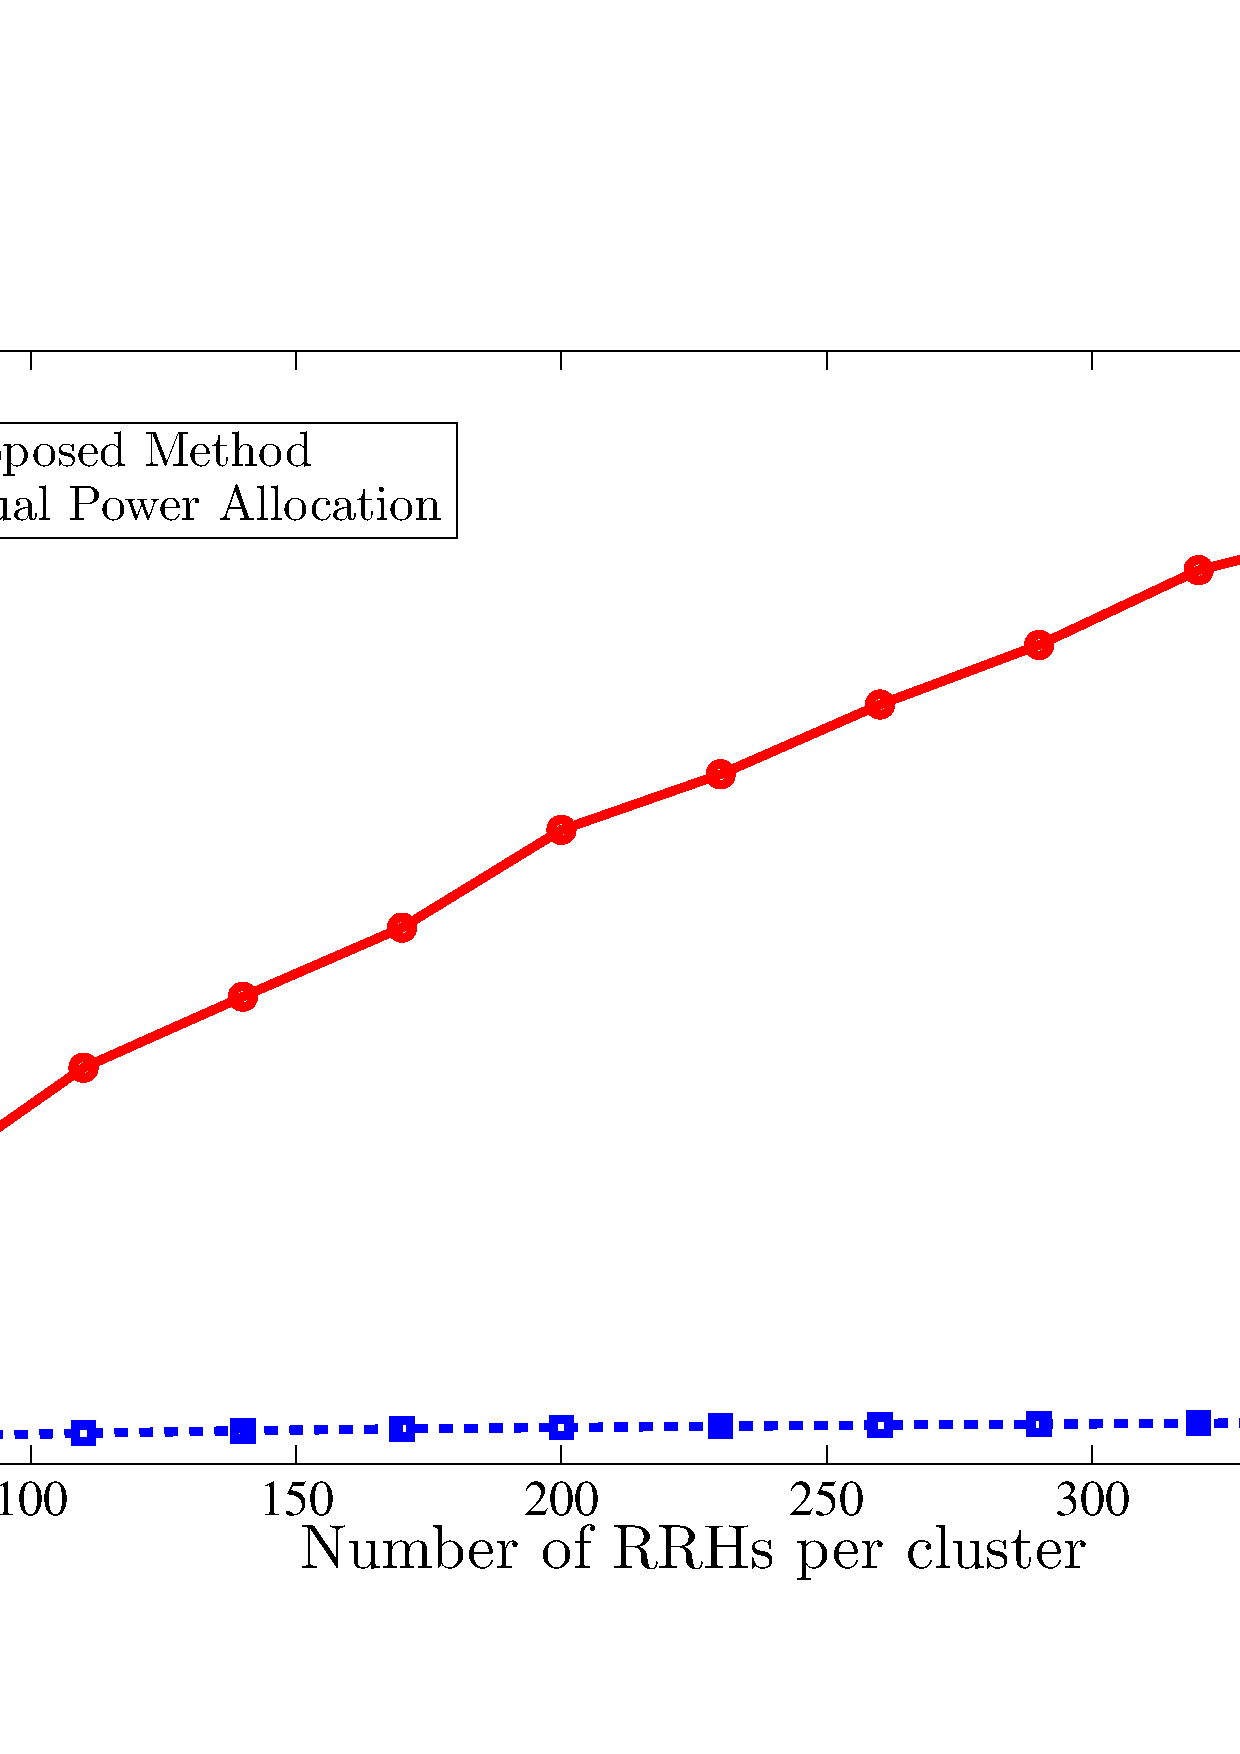
\includegraphics[width=\columnwidth]{n123}
  \caption{Energy efficiency vs number of RRH for Optimized and Equal Power Allocation, plotted for parameters given in Table I with $U_s=8$.}
  \label{fig:nem1}
\end{figure}


In Fig. \ref{fig:nem2}, EE of the proposed iterative algorithm and equal power allocation is depicted with different number of UE in each cluster. It is shown that the iterative algorithm outperforms  again.
Since by increasing the number of UE in each cluster, interference also increased. So the system performance is decreased according to the increase in number of UE.  
  \begin{figure}
  \centering
    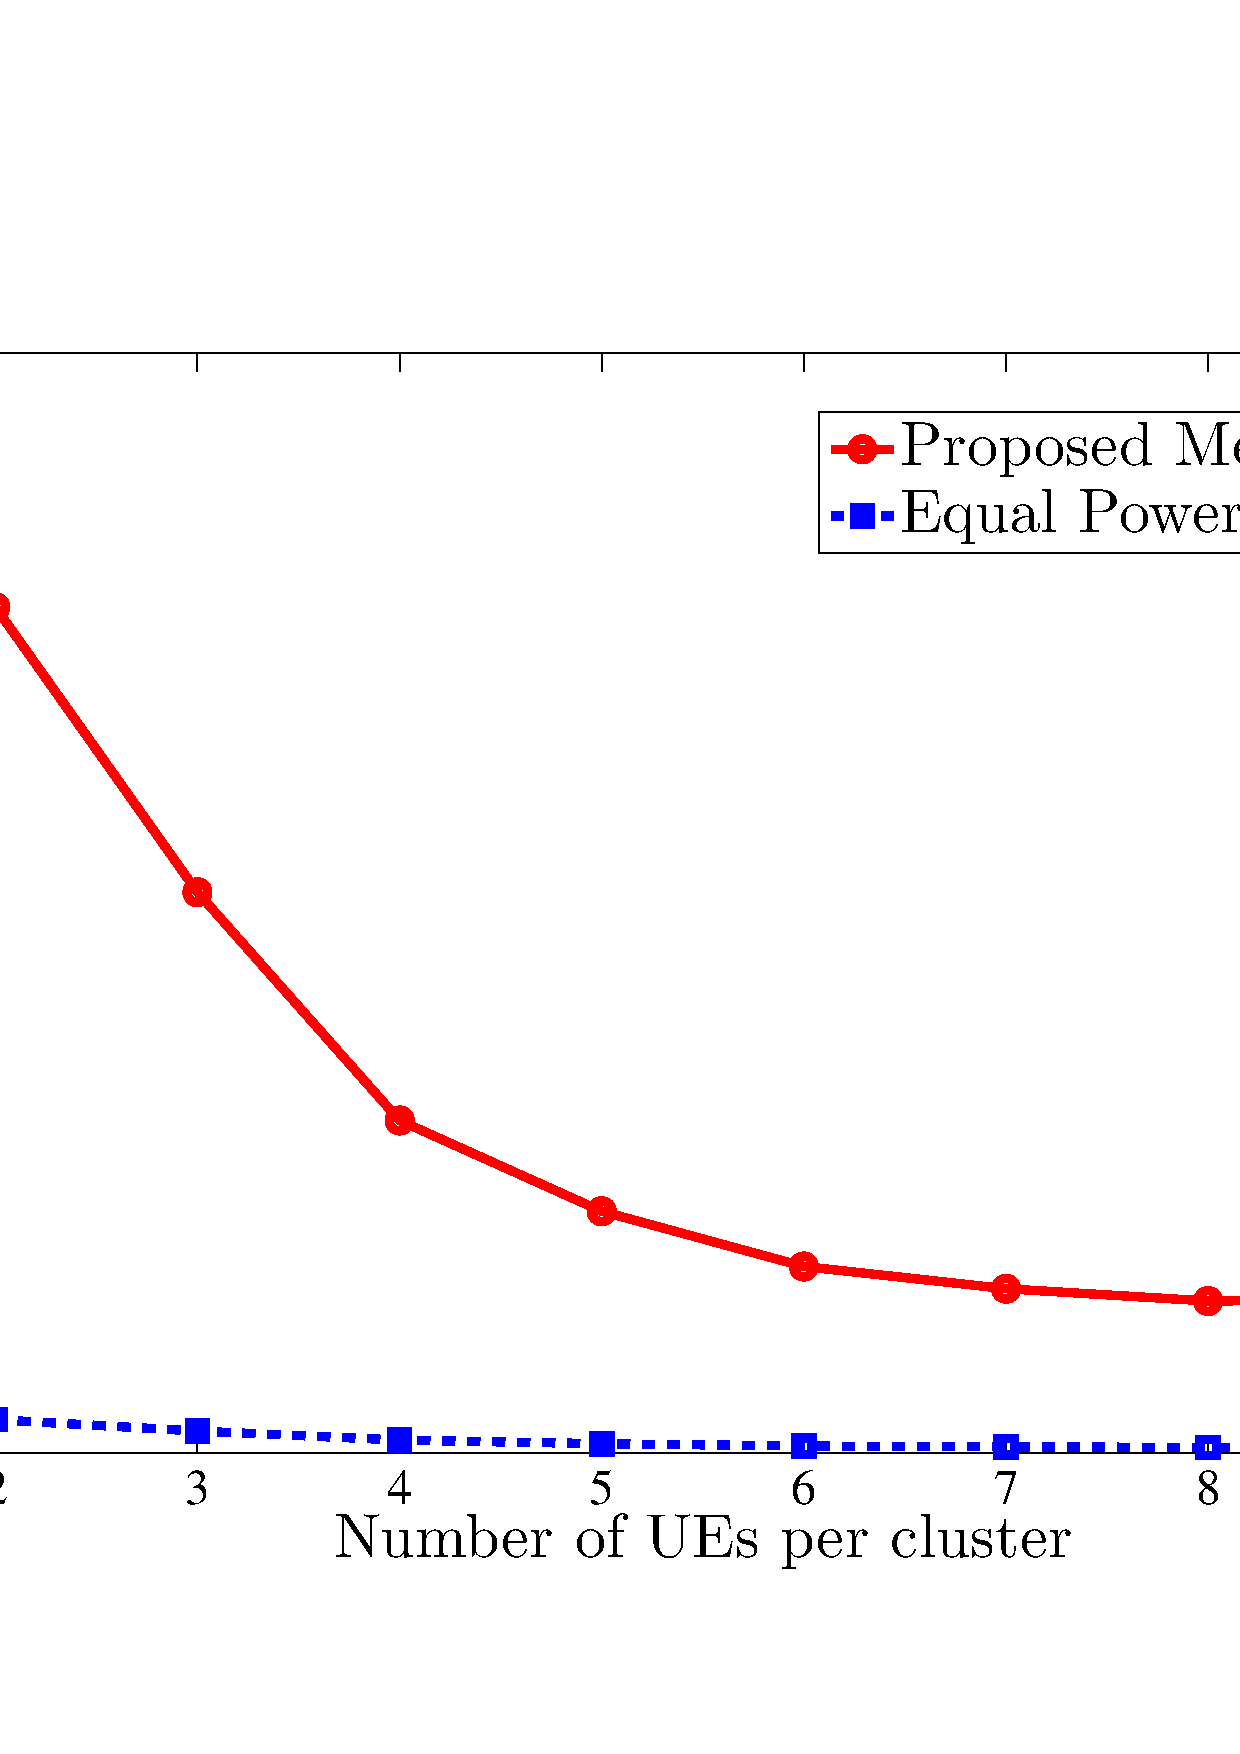
\includegraphics[width=\columnwidth]{ue}
  \caption{Energy efficiency vs number of UE for Optimized and Equal Power Allocation, plotted for parameters given in Table I with $M_s=30$.}
  \label{fig:nem2}
\end{figure}
%\bibliographystyle{ieeetr}
%\bibliography{bib1}
%\setLTRbibitems
\begin{figure}
  \centering
    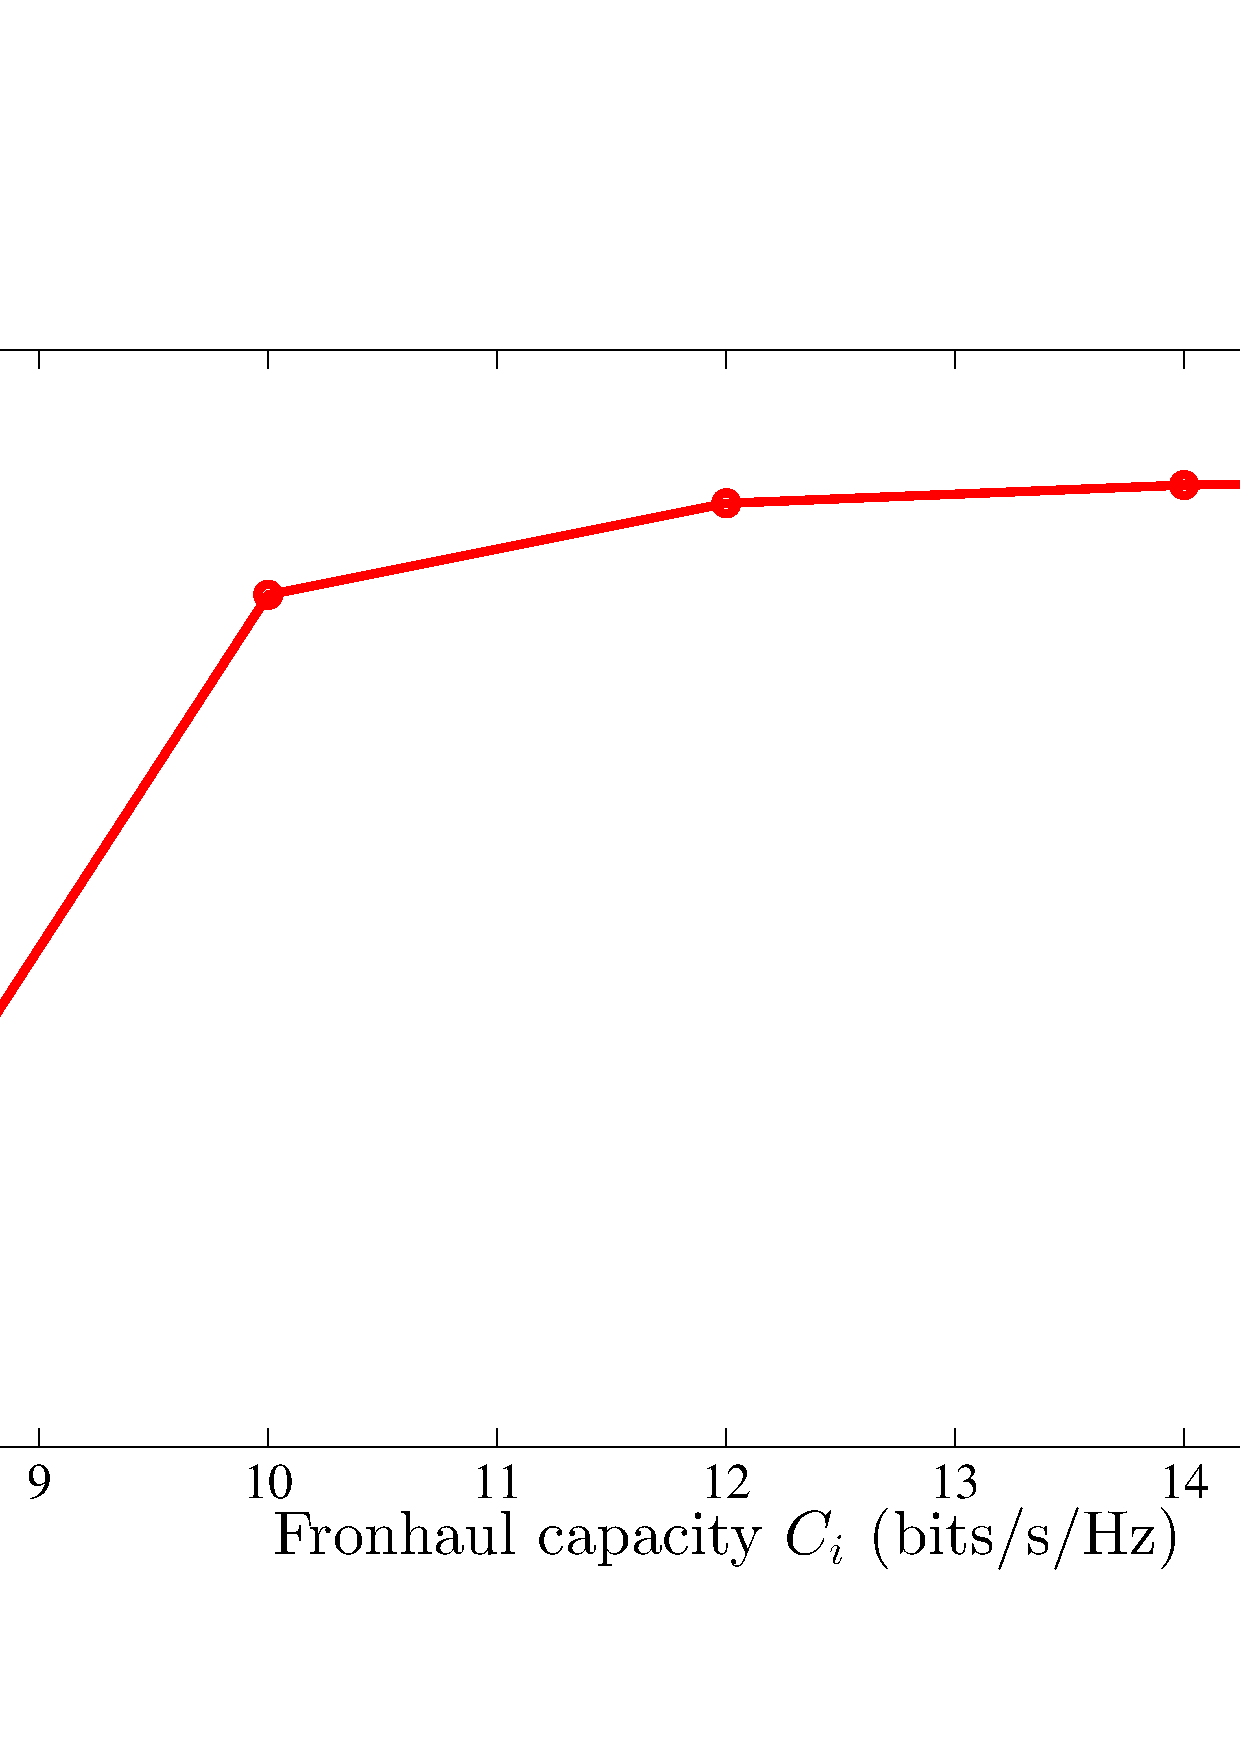
\includegraphics[width=\columnwidth]{c}
  \caption{Energy efficiency vs ${C}^{th} $ constraint with $S =3.Ms= 20, U =3$ }
  \label{fig:nem3}
\end{figure}


In Fig. \ref{fig:nem3}, EE is depicted as a function of the maximum fronthaul link capacity constraint. In this simulation as the capacity  exceeds 12 (bits/s/Hz) , the EE tends to be saturated.
\section{Conclusion}
In this paper, we have focused on optimizing power allocation in downlink of MIMO C-RAN system with limited fronthaul capacity.
 The compressed messages are forwarded via the limited capacity fronthaul links to the RRHs which are clustered into $S$ cluster sets.
The system model is expressed and the problem of maximizing the EE is solved by using an iterative algorithm and Lagrangian function.
Simulation results demonstrate that by increasing the number of RRHs in each cluster, the performance of the system would be enhanced. 
On the other hand, by increasing the number of UE in each cluster, the system performance is reduced.


\bibliographystyle{ieeetr}
\bibliography{m}
 %%
\
\end{document}
